\chapter[Implementation Details for Agentic Logistic Mitigation Framework]{Implementation Details for Agentic Logistic Mitigation Framework}
\sloppy

Detailed information regarding the implementation of the proposed system is provided here. How the system design discussed in previous chapters was transformed into a working solution using appropriate technologies, tools, frameworks, and development practices is explained herein.


\section[Implementation Requirements]{Implementation Requirements}
This section specifies the hardware and software requirements necessary for the development and execution of the proposed system. Establishing a baseline environment ensures that the backend optimization engine, local agentic execution, and frontend leaflet dashboard operate smoothly and without resource bottlenecks.

\subsection[Hardware Requirements]{Hardware Requirements}
\begin{itemize}
\item \textbf{Processor}: Intel Core i5 / AMD Ryzen 5 or equivalent (Minimum); Intel Core i7 / Apple M1/M2 or higher (Recommended for faster multi-tier graph computations).
\item \textbf{RAM}: 8 GB (Minimum); 16 GB or higher (Recommended for handling large NetworkX logistics graphs and local multi-agent processing simultaneously).
\item \textbf{Storage}: 256 GB SSD (Minimum) to store datasets, Python environments, and project files.
\item \textbf{Network}: High-speed, stable internet connection (Crucial for continuous, low-latency API calls to Google Gemini and real-time data ingestion).
\end{itemize}

\subsection[Software Requirements]{Software Requirements}
\begin{itemize}
    \item \textbf{Operating System}: Windows 10/11, macOS, or Linux (Ubuntu 20.04+).
    \item \textbf{Programming Language}: Python 3.9 or higher
    \item \textbf{AI and LLM Services}: Google Gemini API (for core natural language reasoning and agent logic).
    \item \textbf{Agentic Frameworks}: CrewAI and LangChain (for orchestrating the multi-agent system and tool calling).
    \item \textbf{Mathematical and Graph Modeling}: NetworkX (for building the Multi-Tier Logistics Digital Twin), alongside Pandas and NumPy for data structuring.
    \item \textbf{Visualization}: Tableau (for the interactive What-If scenario dashboard).
    \item \textbf{Development Environment (IDE)}: Visual Studio Code (VS Code)
    \item \textbf{Frontend tools}: React (v19.x), Axios (v1.x), Leaflet and React-Leaflet (v5.x)
    \item \textbf{Version Control}: Git and GitHub
\end{itemize}


\subsection[Development Environment]{Development Environment}

The development setup is designed to support the local execution, integration testing, and debugging of the digital twin application.

\begin{itemize}
    \item \textbf{Development Workflow:} \\
    The development flow uses a standard client-server iteration cycle. Backend algorithmic changes are written in Python and instantly exposed via FastAPI hot-reloading. The frontend React interface consumes these APIs, validating structural updates on local development ports (e.g., \texttt{http://localhost:5173}).
    \item \textbf{Project Structure:} \\
    The workspace is organized into isolated directories:
    \begin{itemize}
        \item \texttt{/logistics\_app\_backend/}: Hosts backend application logic (\texttt{main.py}), local environment settings, and API routes.
        \item \texttt{/logistics\_app\_frontend/}: Contains the React project source code, dependencies (\texttt{package.json}), and build assets.
        \item \texttt{/network\_model/}: Stores static graph topologies and network definition files.
        \item \texttt{/engine/}: Contains the core mathematical calculation scripts (Dijkstra algorithm executions and shock calculators).
    \end{itemize}
    \item \textbf{Environment Configuration:} \\
    Secret keys (such as the Gemini API credentials) and server settings are managed using a \texttt{.env} file loaded into the system process at runtime, preventing configuration details from being committed to the repository.
    \item \textbf{Build and Execution Environment:}
    \begin{itemize}
        \item \textbf{Backend:} Executed via Python 3.10+ virtual environments (\texttt{venv}), with package installations managed by \texttt{pip}. The REST API runs locally using \texttt{uvicorn} as the ASGI web server.
        \item \textbf{Frontend:} Built and served locally using Vite's development server, which handles fast ESbuild transpiling.
    \end{itemize}
    \item \textbf{Testing and Debugging Environment:}
    \begin{itemize}
        \item Interactive script executions (\texttt{python main.py}) are tested using API clients like \textbf{Postman} or \textbf{cURL} to verify route payloads.
        \item Web console logs (Chrome Developer Tools) are used to track Leaflet map rendering issues and evaluate React state modifications.
    \end{itemize}
\end{itemize}

\section[Implementation Tool Features]{Implementation Tool Features}
The core language, library, and framework features leveraged during implementation are presented in this section. Modern software engineering relies heavily on using built-in language properties and optimized open-source libraries to manage complex graph traversals and asynchronous agent execution. The key features of our stack are described below.

\subsection[Programming Language Features]{Programming Language Features}

\subsubsection{Python}
\begin{itemize}
    \item \textbf{Dynamic Typing with Optional Type Hinting:} Offers development speed while allowing static checking via typing annotations (e.g., \texttt{list[dict]}), reducing variable errors.
    \item \textbf{First-Class Functions:} Functions can be treated as arguments, enabling the system to pass mathematical tools (\texttt{CheckInventoryTool}, \texttt{DijkstraOptimalRouteTool}) directly to \texttt{CrewAI} tasks.
    \item \textbf{Cross-Platform Compatibility:} The standard libraries (\texttt{pathlib}, \texttt{json}, \texttt{math}) compile and execute identically on Windows, Linux, and macOS.
    \item \textbf{Automatic Memory Management:} Internal garbage collection simplifies memory operations when dynamically modifying and discarding large graph models in memory.
\end{itemize}

\subsubsection{JavaScript (ES6+ / JSX)}
\begin{itemize}
    \item \textbf{Asynchronous Event Loop:} Supports non-blocking operations (\texttt{async/await}), ensuring that long-running agent requests do not freeze the browser UI.
    \item \textbf{Component Declarativity (JSX):} Allows nesting HTML structures directly inside JavaScript logic, creating self-contained UI modules that represent network nodes and paths.
\end{itemize}

\subsection[Framework and Library Features]{Framework and Library Features}

\subsubsection{FastAPI (Backend Web Framework)}
\begin{itemize}
    \item \textbf{Asynchronous Support:} Built on ASGI standards, allowing high-concurrency requests.
    \item \textbf{Automatic Documentation:} Instantly compiles OpenAPI/Swagger documentation pages (\texttt{/docs}) for API testing.
    \item \textbf{Pydantic Validation:} Ensures incoming POST bodies are type-safe before internal execution.
\end{itemize}

\subsubsection{CrewAI (Agentic Orchestration Framework)}
\begin{itemize}
    \item \textbf{Role-Playing Architecture:} Allows setting custom goals, backstories, and LLM temperature constraints for individual agents.
    \item \textbf{Collaborative Chains:} Pipes task contexts sequentially, feeding output states (such as Dijkstra calculation results) directly into downstream tasks.
\end{itemize}

\subsubsection{NetworkX (Graph Theory Library)}
\begin{itemize}
    \item \textbf{Complex Graph Structures:} Provides class definitions for Directed Multigraphs (\texttt{DiGraph}).
    \item \textbf{Optimized Math Solvers:} Implements a highly efficient Dijkstra pathfinder to instantly resolve alternative lanes during disruptions.
\end{itemize}

\subsubsection{React (Frontend UI Framework)}
\begin{itemize}
    \item \textbf{State Hooks (\texttt{useState}, \texttt{useEffect}):} Automatically triggers map and dashboard updates when data is received from backend APIs.
    \item \textbf{Virtual DOM:} Minimizes layout shifts, allowing the UI to render dynamic animations smoothly.
\end{itemize}

\subsection[Database Features]{Database Features}

The system relies on a \textbf{NoSQL Document Store} consisting of structured JSON documents to represent operational states:

\begin{itemize}
    \item \textbf{Data Storage Capabilities:} Stores hierarchical, unstructured, or semi-structured data (nodes array, edges array, mapping keywords) without requiring rigid schema alterations.
    \item \textbf{Query Handling Support:} Graph nodes are queried in $O(1)$ constant time using Python dictionary hashing lookup schemes.
    \item \textbf{Scalability and Performance Features:} In-memory graph loading allows the system to execute path queries and shock weight calculations within milliseconds, bypassing standard database connection pooling latencies.
    \item \textbf{Data Management Capabilities:} Simple file-based configuration makes it easy to back up, restore, and transfer the entire logistics network state by copying text files.
\end{itemize}

\subsection[Version Control and Supporting Tools]{Version Control and Supporting Tools}

\begin{itemize}
    \item \textbf{Version Control System (Git):} Used to track incremental code changes, manage code branches, and merge frontend/backend components.
    \item \textbf{Collaboration Tools (GitHub):} Serves as the central repository host, allowing developers to review code revisions, document issues, and manage project milestones.
    \item \textbf{Testing and Debugging Tools:}
    \begin{itemize}
        \item \textbf{Chrome DevTools:} Used to inspect network request-response payloads and debug React rendering performance.
        \item \textbf{Uvicorn Console Logs:} Outputs color-coded real-time backend API requests and stack traces.
    \end{itemize}
    \item \textbf{Build Automation Tools (\texttt{npm} / Vite):} Manages package compiling, optimizes JavaScript assets, and minimizes code size for frontend builds.
\end{itemize}
\section[Platform Selection and environment]{Platform Selection and environment}
This section discusses the platform selection and operating environment chosen for the proposed system. Designing a real-time digital twin requires careful balancing of client-side responsiveness and backend computational throughput. The operational runtime constraints and hosting choices are detailed below.
\subsection[Platform Selection]{Platform Selection}
The system is developed as a Web-Based Client-Server Application. This platform configuration was selected over desktop or standalone alternatives based on the following engineering rationales:

\begin{itemize}
    \item \textbf{Compatibility with Project Requirements:} A logistics digital twin requires real-time geospatial visualization and interactive simulation controls. A web-based platform allows integrating open-source mapping engines (Leaflet) directly into the UI, rendering complex path coordinate shifts instantly inside the browser.
    \item \textbf{Performance Considerations:} By splitting the application into a frontend client and a backend server, heavy computational tasks—such as executing Dijkstra’s pathfinder on dynamic graphs and orchestrating CrewAI reasoning loops—are offloaded to the backend. The client machine's resources are dedicated exclusively to UI rendering, preventing layout freezes.
    \item \textbf{Scalability:} A web platform facilitates easy scaling. The backend can be containerized and hosted on cloud environments to scale horizontally, while multiple client devices (logistics managers, warehouse operators) can access the dashboard simultaneously via web browsers.
    \item \textbf{Ease of Development:} Web standards (React, JavaScript, CSS) provide robust libraries for UI animations and responsive grids. This allows for rapid iteration of layout elements (such as the glassmorphic design and control panels) without rebuilding platform-specific installers.
    \item \textbf{Resource Availability:} Web development enjoys extensive documentation and open-source packages (e.g., standard mapping wrappers, HTTP client managers, and charting libraries), reducing integration overheads.
\end{itemize}

\subsection[Operating Environment]{Operating Environment}
The runtime and execution specifications of the system are defined as follows:

\begin{itemize}
    \item \textbf{Supported Operating Systems:}
    \begin{itemize}
        \item \textbf{Development and Hosting Server:} Cross-platform compatibility. Supported on Windows (10/11), macOS, and Linux (Ubuntu 20.04+).
        \item \textbf{Client Devices:} Any OS equipped with a modern web browser, including Windows, macOS, Linux, iOS, and Android.
    \end{itemize}
    \item \textbf{Runtime Environment:}
    \begin{itemize}
        \item \textbf{Backend Runtime:} Python v3.10 or higher.
        \item \textbf{Frontend Compilation:} Node.js v18.x or v20.x (LTS) environment for bundling assets during development.
    \end{itemize}
    \item \textbf{Browser Compatibility:} The frontend interface is compatible with modern browsers supporting ES6 Modules and HTML5 Canvas rendering:
    \begin{itemize}
        \item Google Chrome (v90+)
        \item Microsoft Edge (v90+)
        \item Mozilla Firefox (v88+)
        \item Apple Safari (v14+)
    \end{itemize}
    \item \textbf{Client-Server Architecture:} The application runs in a distributed environment:
    \begin{itemize}
        \item \textbf{Client:} The React browser application handles user events and visualizes telemetry data.
        \item \textbf{Server:} The FastAPI backend serves REST APIs, loads graph databases in memory, and interfaces with the Gemini LLM.
    \end{itemize}
    \item \textbf{Network Requirements:}
    \begin{itemize}
        \item \textbf{Local Connection:} Low-latency HTTP/JSON connection on local ports (e.g., 5173 for the client and 8000 for the server).
        \item \textbf{External WAN Connection:} Mandatory high-speed internet connection on the server host to communicate with the remote Google Gemini API endpoints for agentic operations.
    \end{itemize}
\end{itemize}
\section[Coding Standards and Development Practices]{Coding Standards and Development Practices}
The coding standards, development conventions, and maintenance strategies followed during the project lifecycle are presented in this section. Adhering to structured naming conventions and separation of concerns is essential to ensure that the codebase remains maintainable, legible, and extensible.

\subsection[Development Best Practices]{Development Best Practices}
The development of the Logistics Digital Twin system incorporated several core software engineering principles and best practices:

\begin{itemize}
    \item \textbf{Modular Programming Approach:} Division of operations into isolated modules (e.g., separating semantic parsing from graph routing).
    \item \textbf{Code Reusability Practices:} Implementation of generic utilities and shared agentic tools.
    \item \textbf{Proper Indentation and Formatting:} Adherence to standard style guides (PEP 8 for Python; ESLint and Prettier for JavaScript/React).
    \item \textbf{Error Handling and Exception Management:} Use of structured try-except blocks and fallback recovery logic.
    \item \textbf{Incremental Testing and Debugging:} Component-level testing before full integration.
    \item \textbf{Code Optimization Techniques:} In-memory graph loading and optimized token prompts to reduce latency.
    \item \textbf{Use of Version Control Systems:} Version tracking and code synchronization using Git.
    \item \textbf{DRY Principle (Don’t Repeat Yourself):} Consolidating repeated calculations into utility packages.
    \item \textbf{Separation of Concerns:} Isolation of UI state, API routing, network models, and agent tasks.
    \item \textbf{Logging and Debugging Practices:} Console logging of application events and API statuses.
\end{itemize}

\subsection[Naming Conventions]{Naming Conventions}
To maintain consistency across both the Python backend and JavaScript/React frontend, the following naming standards were strictly applied:

\begin{itemize}
    \item \textbf{Files:}
    \begin{itemize}
        \item \textbf{Python:} Snake case (e.g., \texttt{build\_network\_model.py}, \texttt{execution\_engine.py}).
        \item \textbf{JavaScript/React:} Pascal case for components (e.g., \texttt{App.jsx}); camel case or kebab case for assets and styling (e.g., \texttt{index.css}).
        \item \textbf{Configurations:} Snake case (e.g., \texttt{network\_topology.json}).
    \end{itemize}
    \item \textbf{Variables:}
    \begin{itemize}
        \item \textbf{Python:} Snake case (e.g., \texttt{shocked\_graph}, \texttt{delta\_days}).
        \item \textbf{JavaScript:} Camel case (e.g., \texttt{optimization}, \texttt{strategy}, \texttt{loading}).
    \end{itemize}
    \item \textbf{Functions:}
    \begin{itemize}
        \item \textbf{Python:} Snake case (e.g., \texttt{dijkstra\_best\_path()}, \texttt{apply\_shock()}).
        \item \textbf{JavaScript:} Camel case (e.g., \texttt{handleOptimize()}, \texttt{getPathCoords()}).
    \end{itemize}
    \item \textbf{Classes:}
    \begin{itemize}
        \item Pascal case across all languages (e.g., \texttt{InventoryManager}, \texttt{MapFocus}).
    \end{itemize}
    \item \textbf{Constants:}
    \begin{itemize}
        \item Screaming snake case across all languages (e.g., \texttt{UNIT\_HOLDING\_COST}, \texttt{API\_BASE}, \texttt{COORDS}).
    \end{itemize}
    \item \textbf{Database Tables and Fields (JSON Property Keys):}
    \begin{itemize}
        \item Snake case for attributes (e.g., \texttt{node\_id}, \texttt{transit\_time}, \texttt{freight\_cost}, and \texttt{severity\_multiplier}).
    \end{itemize}
\end{itemize}

\subsection[Code Maintainability Practices]{Code Maintainability Practices}
To ensure the codebase remains extensible and clean over its lifecycle, the following maintainability strategies were prioritized:

\begin{itemize}
    \item \textbf{Modular Organization of Code:} Locating the graph logic (\texttt{network\_model}), routing calculations (\texttt{engine}), server routes (\texttt{logistics\_app\_backend}), and user interface (\texttt{logistics\_app\_frontend}) in distinct, independent folders.
    \item \textbf{Reusable Components:} Encapsulating specific frontend features (such as Leaflet map views or metrics blocks) and backend tools (such as inventory query APIs) into reusable units.
    \item \textbf{Configuration Management:} Storing operational constants, network topology edges, and risk rules in external JSON documents to avoid hardcoding values inside routing scripts.
    \item \textbf{Logging and Debugging Support:} Implementing structured terminal printing and execution trace logs in FastAPI to simplify diagnostics.
    \item \textbf{Separation of Functionality:} Separating presentation logic (HTML/CSS layout) from business logic (Python algorithms) to allow front-end and back-end updates to occur independently.
\end{itemize}
\section[Module Implementation and Integration]{Module Implementation and Integration}
This section describes the detailed implementation and integration methodologies used to connect the system's modular components. We detail the technical functionality of each module, the data exchange protocols, database connectivity mechanisms, and transaction safety measures used to build a unified system.

\subsection[Module Implementation Overview]{Module Implementation Overview}
The implementation details of the major system modules are structured as follows:

\begin{enumerate}[label=\Roman*.]
    \item \textbf{Friction Sentry Module}
    \begin{itemize}
        \item \textbf{Functionality Implemented:} Evaluates incoming simulated shock descriptions, parses their locations and types, and uses lookup tables to identify the direct and cascading cost and time multipliers.
        \item \textbf{Technologies Used:} Python, standard JSON parser library.
        \item \textbf{Internal Processing Logic:} Reads incoming shock parameters, scans the \texttt{signal\_type\_rules} index in the rules library, propagates severity factors to downstream nodes, and formats the output into a standardized JSON shock payload.
        \item \textbf{Interaction with Other Modules:} Exports the structured shock payload to the API server, which forwards it to the \textbf{Networked Digital Twin}.
    \end{itemize}

    \item \textbf{Networked Digital Twin Module}
    \begin{itemize}
        \item \textbf{Functionality Implemented:} Represents the physical logistics topology as a network graph, applies shock weights, and calculates inventory depletion parameters.
        \item \textbf{Technologies Used:} Python, \texttt{networkx} library.
        \item \textbf{Internal Processing Logic:} Instantiates a directed graph using topological data. Upon receiving a shock payload, it dynamically modifies edge attributes (\texttt{cost} and \texttt{transit\_time}) and computes market Days of Cover ($DoC$) using current stock levels and demand curves.
        \item \textbf{Interaction with Other Modules:} Receives input from the \textbf{Friction Sentry} via the API server, and serves the active shocked graph data to the \textbf{Logistics Optimizer}.
    \end{itemize}

    \item \textbf{Logistics Optimizer Module}
    \begin{itemize}
        \item \textbf{Functionality Implemented:} Performs shortest-path routing optimization and coordinates multi-agent decision chains to manage inventory.
        \item \textbf{Technologies Used:} Python, \texttt{CrewAI} orchestration framework, Google Gemini API client.
        \item \textbf{Internal Processing Logic:} Invokes a dynamic Dijkstra pathfinder on the weighted shocked graph. If inventory evaluations indicate an impending stockout, the module initiates a CrewAI task sequence, prompting agents to query tools and trigger emergency restocking actions.
        \item \textbf{Interaction with Other Modules:} Accepts shocked network graphs from the \textbf{Networked Digital Twin} and returns recommendation payloads to the \textbf{Interactive Dashboard} via FastAPI.
    \end{itemize}

    \item \textbf{Interactive Dashboard Module}
    \begin{itemize}
        \item \textbf{Functionality Implemented:} Maps geographical coordinates, renders shipping lane polylines, and displays performance metrics.
        \item \textbf{Technologies Used:} React, JavaScript (ES6+), Leaflet, Lucide-React.
        \item \textbf{Internal Processing Logic:} Resolves node names to coordinate arrays, listens to state changes to toggle route polylines (dashed for baseline, bold for optimized), and updates KPI widgets based on server response data.
        \item \textbf{Interaction with Other Modules:} Communicates with the backend API by transmitting user strategy selections and receiving optimization payloads.
    \end{itemize}
\end{enumerate}

\subsection[Integration of Modules]{Integration of Modules}
The integration strategy adopts a \textbf{Sandwiched API integration} pattern (Figure \ref{fig:module_integration}), connecting the frontend user interface and the computational backend modules through a central controller.

\begin{figure}[htbp]
    \centering
    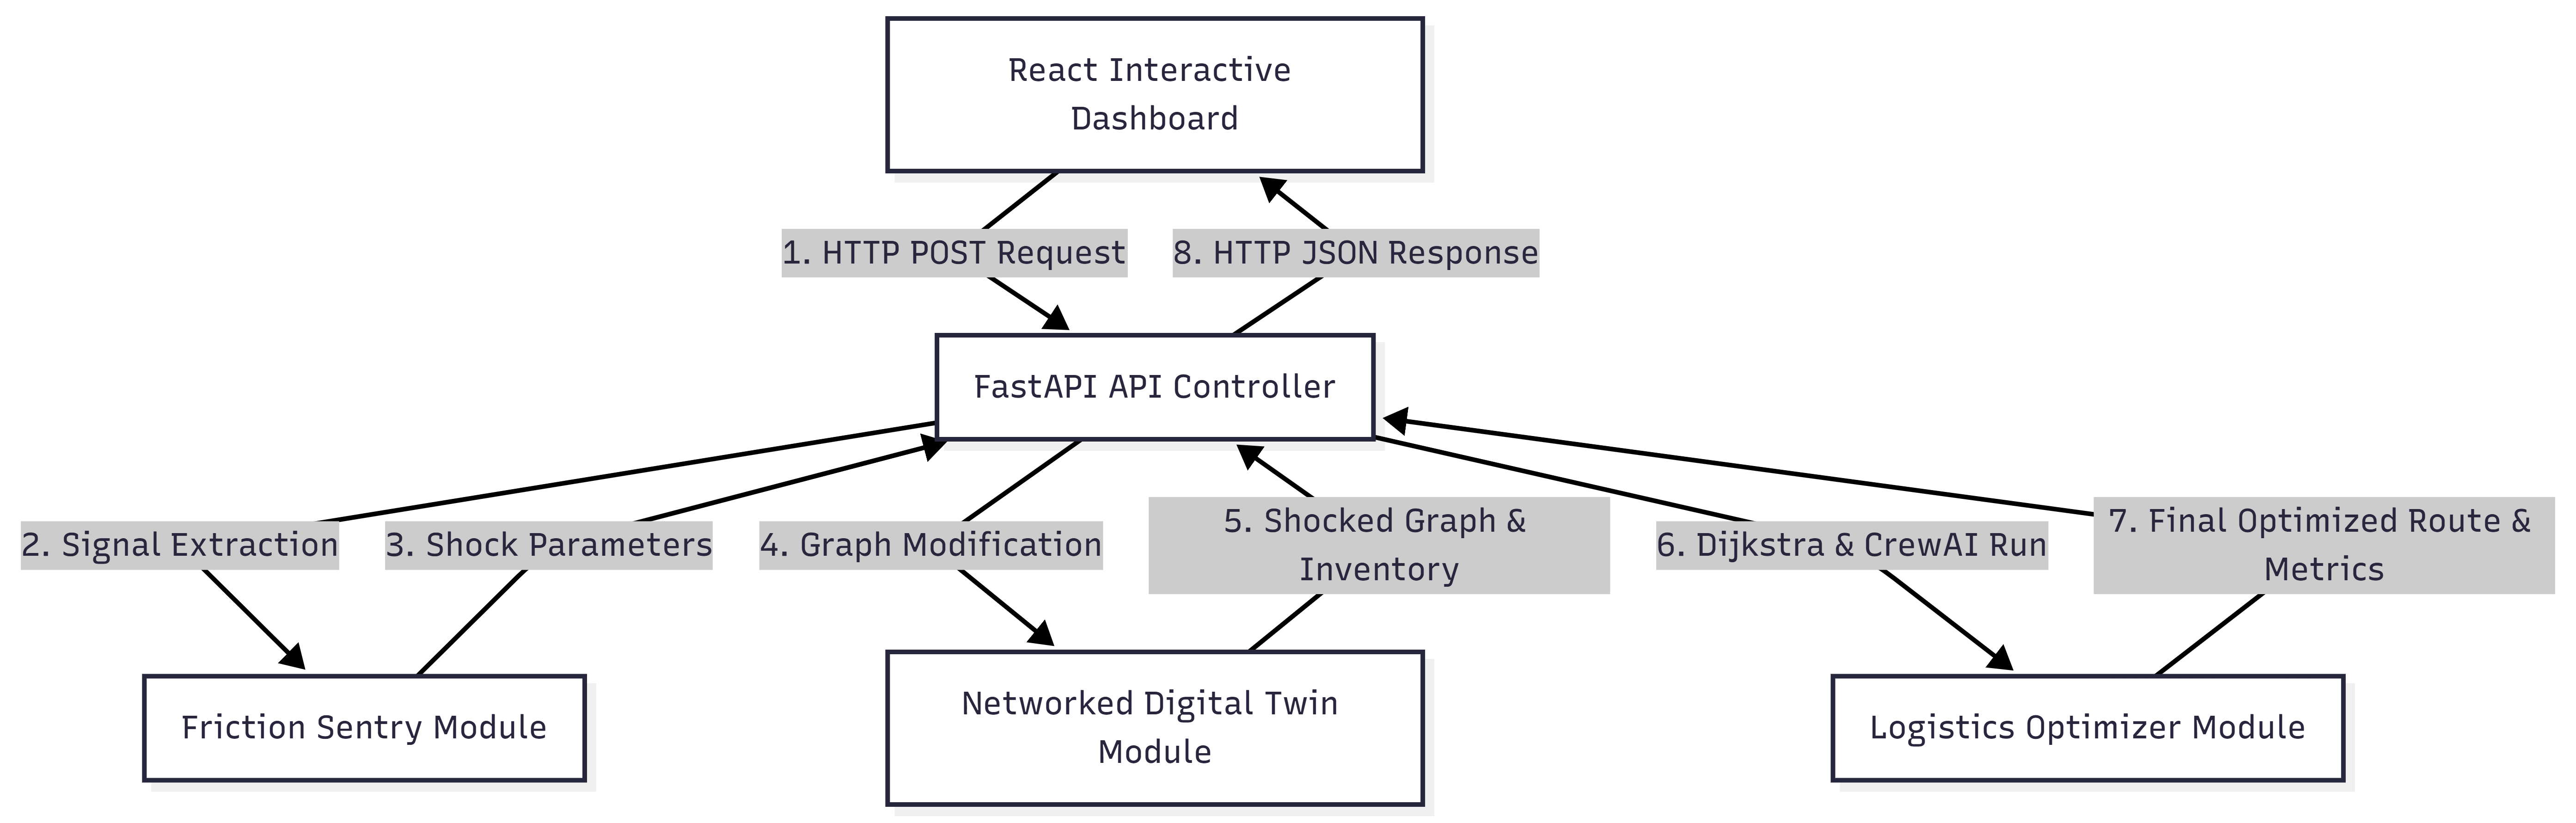
\includegraphics[width=\textwidth]{Figures/Module integration.png}
    \caption{Module Integration and Data Flow}
    \label{fig:module_integration}
\end{figure}

\begin{itemize}
    \item \textbf{Inter-Module Communication:} Performed locally via standard function calls and class instantiation in Python, and remotely using HTTP request-response actions between the client and server.
    \item \textbf{Data Exchange Mechanisms:} Structured \textbf{JSON (JavaScript Object Notation)} serves as the universal data contract. All modules consume and output validated JSON objects matching predefined schemas.
    \item \textbf{Request-Response Workflow:} 
    \begin{enumerate}[label=(\roman*)]
        \item The user selects a routing strategy (e.g., cost) and clicks the action trigger on the client dashboard.
        \item The browser dispatches a POST request to \texttt{/api/optimize}.
        \item The server runs the backend pipeline (Sentry $\rightarrow$ Digital Twin $\rightarrow$ Optimizer) synchronously.
        \item The server returns the compiled payload containing path coordinates, delta metrics, and agent summaries to the client to update the UI.
    \end{enumerate}
\end{itemize}

\subsection[Database Connectivity and Data Handling]{Database Connectivity and Data Handling}
The application adopts a light, high-performance in-memory database and configuration mapping approach:

\begin{itemize}
    \item \textbf{Database Connection Strategy:} 
    Instead of utilizing persistent external database connections (such as SQL pools), the system reads locally stored JSON document databases directly into memory. Connection handles are open-and-close operations executing on the local filesystem, avoiding connection timeouts or pool exhaustions.
    \item \textbf{Data Storage and Retrieval:} 
    \begin{itemize}
        \item Network properties and rules are retrieved by deserializing \texttt{network\_topology.json} and \texttt{semantic\_mapping\_rules.json} into nested Python dictionaries at server startup.
        \item Spatial node coordinates are stored in a static key-value map within both the client and server configurations.
    \end{itemize}
    \item \textbf{Query Execution Process:} 
    Queries for node details, edge values, or matching rules are handled via direct hash map lookups (e.g., \texttt{rules[signal\_type\_rules][signal\_type]}), executing in $O(1)$ constant time.
    \item \textbf{Transaction Handling:} 
    Since the operational digital twin does not require multi-user transactional writes to a database, operations are read-only. Updates to graph weights and inventory counts during a shock are managed within isolated, in-memory session instances, removing the need for transaction rollbacks.
    \item \textbf{Data Consistency Management:} 
    To prevent state leakage between simulation runs, the \texttt{InventoryManager} state is re-instantiated and reset to baseline levels before each new optimization cycle, ensuring consistent and reproducible simulation results.
\end{itemize}
\section[Difficulties Encountered and Strategies Used to Tackle Them]{Difficulties Encountered and Strategies Used to Tackle Them}
The technical and operational difficulties encountered during the implementation phase, along with the strategies adopted to address them, are discussed in this section. Building multi-agent workflows involves managing agent hallucinations, API latencies, and token constraints, which required structured refactoring of the backend.

\subsection[Technical Challenges]{Technical Challenges}
During the implementation of the multi-agent system, the following core technical challenge was encountered:

\begin{itemize}
    \item \textbf{Cognitive Agent Output Hallucinations:}
    \begin{itemize}
        \item \textbf{The Problem:} In the initial pipeline configuration, the \textit{SME Communicator Agent} (the final agent in the execution sequence) frequently hallucinated critical numerical values, such as landed costs and transit days.
        \item \textbf{Root Cause:} Under standard \texttt{CrewAI} behavior, only the final task's output is returned to the execution loop by default. Because the preceding tasks (calculated by the \textit{Logistics Optimizer} and \textit{Cost Analyst}) did not explicitly forward their outputs as structured parameters to the final communicator task, the \textit{Communicator Agent} was forced to make assumptions, resulting in numerical hallucinations.
        \item \textbf{Development Complexity:} This created significant complexity because traditional regex parsing or simple string checking on the backend could not validate the truthfulness of these dynamically generated values before they reached the user interface.
    \end{itemize}
\end{itemize}

\subsection[Performance and Scalability Challenges]{Performance and Scalability Challenges}
The primary operational challenges focused on execution delays and network-dependent constraints:

\begin{itemize}
    \item \textbf{LLM API Response Latency:}
    \begin{itemize}
        \item \textbf{The Problem:} Multi-agent systems execute tasks sequentially, requiring multiple network roundtrips to the remote Google Gemini API. 
        \item \textbf{Details:} Each agent must generate an internal thought process (chain-of-thought), execute tools, and evaluate outcomes before yielding control. This multi-turn reasoning caused backend response times to stretch from \textbf{10 to 45 seconds} per simulation run under high API loads.
    \end{itemize}
    \item \textbf{Resource Optimization Constraints:} Passing large, unstructured portions of the network topology data to the LLM context window created excessive token consumption, increasing API costs and execution latency.
    \item \textbf{Concurrence and Rate-Limiting:} Simultaneous dashboard requests are constrained by the remote LLM endpoint's maximum requests per minute (RPM) limits, leading to potential connection dropouts.
\end{itemize}

\subsection[Strategies and Solutions Adopted]{Strategies and Solutions Adopted}
To resolve the identified challenges, the architecture was refactored with the following strategies:

\begin{itemize}
    \item \textbf{Context-Linked Prompt Chaining:}
    Tasks were linked explicitly inside the CrewAI execution logic. The Analyst task (\texttt{t2}) was configured with \texttt{context=[t1]} to pass the Optimizer's route parameters to the Analyst. Crucially, the Analyst task prompt was refactored to enforce the forwarding of \texttt{total\_transit\_days} and \texttt{total\_cost\_usd} inside its own expected output.

    \item \textbf{Expected Output Schema Enforcement:}
    Enforced strict output structures using \texttt{expected\_output} criteria. The Analyst and Communicator tasks were instructed to output data strictly inside a standard JSON format containing keys for recommended path, total transit days, total cost, delta metrics, and inventory status. This completely eliminated the Communicator's information gap, forcing it to consume verified parameters from preceding tasks instead of fabricating them.

    \item \textbf{Deterministic Fallback Routing:}
    A programming fail-safe was implemented at the API server layer. If the agentic reasoning pipeline fails to return a valid JSON structure within a specified timeout limit, the server automatically bypasses the LLM layer, executes Dijkstra's algorithm on the database directly, and returns the mathematically validated path to prevent frontend crashes.

    \item \textbf{Context Optimization:}
    Instead of passing the entire network graph, prompts were optimized to only inject the valid list of node IDs and edge routes as a small, structured schema context, significantly reducing token usage and decreasing LLM latency.
\end{itemize}
\section[Summary]{Summary}
This chapter detailed the implementation of the proposed framework, highlighting the use of Python, FastAPI, and CrewAI for the backend, alongside React and Leaflet for the frontend. It discussed the development environment, coding standards, and the strategies used to overcome technical challenges such as API latency and agentic hallucinations. The resulting implementation provides a robust, scalable platform for simulating and mitigating maritime logistics disruptions.










